% This is the Reed College LaTeX thesis template. Most of the work
% for the document class was done by Sam Noble (SN), as well as this
% template. Later comments etc. by Ben Salzberg (BTS). Additional
% restructuring and APA support by Jess Youngberg (JY).
% Your comments and suggestions are more than welcome; please email
% them to cus@reed.edu
%
% See http://web.reed.edu/cis/help/latex.html for help. There are a
% great bunch of help pages there, with notes on
% getting started, bibtex, etc. Go there and read it if you're not
% already familiar with LaTeX.
%
% Any line that starts with a percent symbol is a comment.
% They won't show up in the document, and are useful for notes
% to yourself and explaining commands.
% Commenting also removes a line from the document;
% very handy for troubleshooting problems. -BTS

% As far as I know, this follows the requirements laid out in
% the 2002-2003 Senior Handbook. Ask a librarian to check the
% document before binding. -SN

%%
%% Preamble
%%
% \documentclass{<something>} must begin each LaTeX document
\documentclass[12pt,twoside]{reedthesis}
% Packages are extensions to the basic LaTeX functions. Whatever you
% want to typeset, there is probably a package out there for it.
% Chemistry (chemtex), screenplays, you name it.
% Check out CTAN to see: http://www.ctan.org/
%%
\usepackage{graphicx,latexsym}
\usepackage{amssymb,amsthm,amsmath}
\usepackage{longtable,booktabs,setspace}
\usepackage{chemarr} %% Useful for one reaction arrow, useless if you're not a chem major
\usepackage[hyphens]{url}
\usepackage[page]{appendix}
\usepackage{rotating}
\usepackage{natbib}
\usepackage{pgfplots}
\usepackage{color}
\usepackage{xcolor}
\usepackage{listings}
\usepackage{caption}
\usepackage{subfiles}
% A better code font
\usepackage{inconsolata}
\lstset{
    language=C,
    keywordstyle=\color{blue},
    basicstyle=\footnotesize\ttfamily,
    commentstyle=\color{gray}
}

\DeclareCaptionFont{white}{ \color{white} }
\DeclareCaptionFormat{listing}{
  \colorbox[cmyk]{0.43, 0.35, 0.35,0.01 }{
    \parbox{\textwidth}{\hspace{15pt}#1#2#3}
  }
}
\captionsetup[lstlisting]{ format=listing, labelfont=white, textfont=white, singlelinecheck=false, margin=0pt }

\lstdefinelanguage
   [x64]{Assembler}     % add a "x64" dialect of Assembler
   [x86masm]{Assembler} % based on the "x86masm" dialect
   % with these extra keywords:
   {morekeywords={CDQE,CQO,CMPSQ,CMPXCHG16B,JRCXZ,LODSQ,MOVSXD, %
                  POPFQ,PUSHFQ,SCASQ,STOSQ,IRETQ,RDTSCP,SWAPGS, %
                  MOVAPD,SUBPD,MULSD,SHUFPD,ADDSD,XORPS,SQRTSD, %
                  MOVDDUP,DIVSD,DIVPD,MULPD,ADDPD %
                  rax,rdx,rcx,rbx,rsi,rdi,rsp,rbp, %
                  r8,r8d,r8w,r8b,r9,r9d,r9w,r9b, %
                  r10,r10d,r10w,r10b,r11,r11d,r11w,r11b, %
                  r12,r12d,r12w,r12b,r13,r13d,r13w,r13b, %
                  r14,r14d,r14w,r14b,r15,r15d,r15w,r15b}} % etc.


\pgfplotsset{compat=1.5}
\usepackage[alsoload=astro]{siunitx}
% Comment out the natbib line above and uncomment the following two lines to use the new
% biblatex-chicago style, for Chicago A. Also make some changes at the end where the
% bibliography is included.
%\usepackage{biblatex-chicago}
%\bibliography{thesis}


\usepackage{fbb} % other fonts are available like times, bookman, charter, palatino

\title{N-Body Simulations of Barred Galaxies}
\author{Thomas B Malthouse}
% The month and year that you submit your FINAL draft TO THE LIBRARY (May or December)
\date{Summer 2017}
\division{Mathematics and Natural Sciences}
\advisor{J Powell}
%If you have two advisors for some reason, you can use the following
%\altadvisor{Your Other Advisor}
%%% Remember to use the correct department!
\department{Physics}


\setlength{\parskip}{1.5em}

\DeclareSIUnit[]\solar
{\mathrm{\ensuremath{M}}_\odot}
\DeclareSIUnit[]\year
{\mathrm{\ensuremath{yr}}}

\definecolor{light-gray}{gray}{0.9}
\newcommand\code[1]{\colorbox{light-gray}{\texttt{\textcolor{black}{#1}}}}


%%
%% End Preamble
%%
%% The fun begins:
\begin{document}

  \maketitle
  \frontmatter % this stuff will be roman-numbered
  \pagestyle{empty} % this removes page numbers from the frontmatter

% Acknowledgements (Acceptable American spelling) are optional
% So are Acknowledgments (proper English spelling)
    \chapter*{Acknowledgements}
	I want to thank a few people.

% The preface is optional
% To remove it, comment it out or delete it.
    \chapter*{Preface}
	This is an example of a thesis setup to use the reed thesis document class.



    \chapter*{List of Abbreviations}
		You can always change the way your abbreviations are formatted. Play around with it yourself, use tables, or come to CUS if you'd like to change the way it looks. You can also completely remove this chapter if you have no need for a list of abbreviations. Here is an example of what this could look like:

	\begin{table}[h]
	\centering % You could remove this to move table to the left
	\begin{tabular}{ll}
		\textbf{ABC}  	&  American Broadcasting Company \\
		\textbf{CBS}  	&  Columbia Broadcasting System\\
		\textbf{CDC}  	&  Center for Disease Control \\
		\textbf{CIA}  	&  Central Intelligence Agency\\
		\textbf{CLBR} 	&  Center for Life Beyond Reed\\
		\textbf{CUS}  	&  Computer User Services\\
		\textbf{FBI}  	&  Federal Bureau of Investigation\\
		\textbf{NBC}  	&  National Broadcasting Corporation\\
	\end{tabular}
	\end{table}


    \tableofcontents
% if you want a list of tables, optional
    \listoftables
% if you want a list of figures, also optional
    \listoffigures

% The abstract is not required if you're writing a creative thesis (but aren't they all?)
% If your abstract is longer than a page, there may be a formatting issue.
    \chapter*{Abstract}
	The preface pretty much says it all.

	\chapter*{Dedication}
	You can have a dedication here if you wish.

  \mainmatter % here the regular arabic numbering starts
  \pagestyle{fancyplain} % turns page numbering back on

%The \introduction command is provided as a convenience.
%if you want special chapter formatting, you'll probably want to avoid using it altogether

% Bring in the introduction, from a separate file, to simplify things and make this file shorter.
\subfile{introduction.tex}

% Do the same for each chapter.
\subfile{optimizations.tex}


\subfile{conclusion.tex}


%If you feel it necessary to include an appendix, it goes here.
\begin{appendices}
    \chapter{}
        \section{The Hubble Classification System} \label{hubble-fork}
            The Hubble Classification System, or Hubble Sequence, is the most commonly used scheme for classifying galaxies. Nicknamed \emph{The Fork}, it goes from elliptical galaxies on the left, to the two kinds (barred and unbarred) of spiral galaxies on the right.

            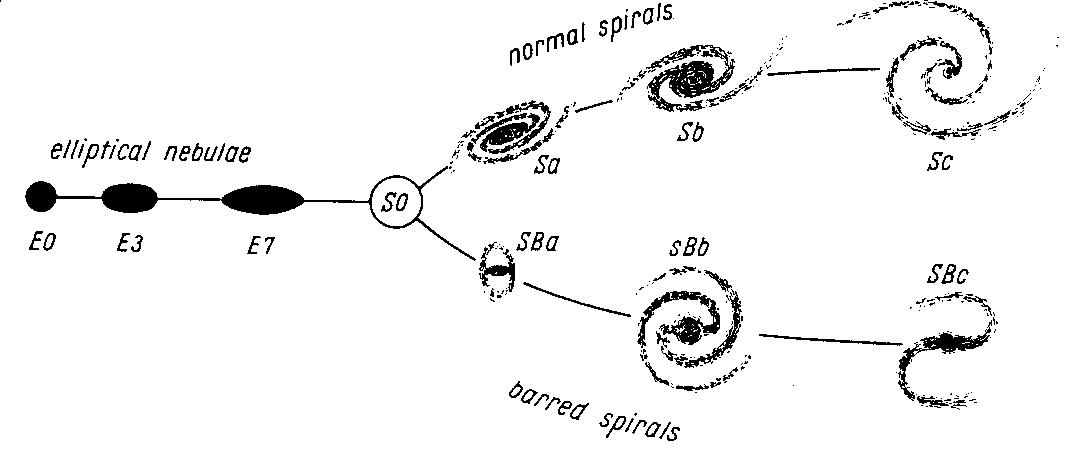
\includegraphics[width=\textwidth]{imgs/hubble_seq}
            \emph{Image courtesy Allan Sandage/CalTech}


        \section{C Language Resources} \label{C-resources}
        \begin{itemize}
            \item \emph{Learn C the Hard Way: Practical Exercises on the Computational Subjects You Keep Avoiding (Like C)}
            ---A good introduction to writing simple, useful C programs. Often breaks with tradition, but always for the better.

            \url{http://www.indiebound.org/book/9780321884923}

            \item \emph{C in a Nutshell}
            ---A massive, 824 page book, that has everything you could ever want to know about using the C language

            \url{http://www.indiebound.org/book/9781491904756}

            \item \emph{21st Century C}
            ---A guide to using a language designed in 1970, in 2017. Most useful if you already have an understanding of C.

            \url{http://www.indiebound.org/book/9781491903896}

            \item \emph{The C Programming Language}
            ---An absolute classic, written by the designers of the language. This book isn't all that useful for \emph{learning} modern C, but it sheds light on the reasons the language was designed the way it was.

            \url{http://www.indiebound.org/book/9780131103627}

            \item \emph{Build your own Lisp}
            ---Learn C by writing an interpreter for the Lisp language. A complete guide to a really fun and useful project. Available both online and as a printed book.

            \url{http://www.buildyourownlisp.com}

            \url{http://www.indiebound.org/book/9781501006623}
        \end{itemize}
\end{appendices}


%This is where endnotes are supposed to go, if you have them.
%I have no idea how endnotes work with LaTeX.

  \backmatter % backmatter makes the index and bibliography appear properly in the t.o.c...

% if you're using bibtex, the next line forces every entry in the bibtex file to be included
% in your bibliography, regardless of whether or not you've cited it in the thesis.
    \nocite{*}

% Rename my bibliography to be called "Works Cited" and not "References" or ``Bibliography''
% \renewcommand{\bibname}{Works Cited}

%    \bibliographystyle{bsts/mla-good} % there are a variety of styles available;
%  \bibliographystyle{plainnat}
% replace ``plainnat'' with the style of choice. You can refer to files in the bsts or APA
% subfolder, e.g.
 \bibliographystyle{APA/apa-good}  % or
 \bibliography{thesis}
 % Comment the above two lines and uncomment the next line to use biblatex-chicago.
 %\printbibliography[heading=bibintoc]

% Finally, an index would go here... but it is also optional.
\end{document}
